%!TEX root = thesis.tex
\chapter{Results}\label{chap:results}
\thispagestyle{plain}

  Equilibrium experiments are useful tools to asses the behavior of glacier models. Thereby, an glacier in equilibrium state is subjected to a step change in cliamte and its evolution is modeled until a new equilibrium is reached. The OGGM provides two climate scenarios for such equilibrium experiments, the \lstinline`ConstantMassBalance` model and the \lstinline`RandomMassBalance` model (see Section~\ref{sub:mass_balance_models_implementation} for implementation details). The experiments are performed on seleceted or all Alpine glaciers, using the HISTALP dataset \citep{Auer2007} as climate input data. The baseline climate for each glacier comes from a 31-year period centered around the \textit{equilibrium year} \tstar. An additional temperature bias of \SI{0}{\celsius}, \SI{-0.5}{\celsius} and \SI{+0.5}{\celsius} results in a neutral, positive and negative step change in mass balance, respectively. The detailed experimental setup can be found in Section...

    The first qualitative conclusions are drawn from the temporal evolution of length, surface area and ice volume. We are looking at selected single glaciers as well as at the regional scale, i.e. at the sum over all glaciers in the HISTALP domain. Scaling methods applied to a single give only an order of magnitude estimation \citep[cf.][Section 8.5]{Bahr2015}, which is accounted for in the following analysis. More quantitative results are drawn from an autocorrelation analysis and a power spectral density analysis, inspired by \citet{Roe2014}. %TODO: not up to date anymore... adjust to new structure!


  \section{Single glacier test case} % (fold)
  \label{sec:single_glacier_test_case_results}

    This first test case is intended to get a feel for the \vas{} model and set the stage for the following experiments. The model estimates the evolution of the Hintereisferner (RGI60-11.00897) over 1000 years for three different climate scenarios: an equilibirum climate, a positive and a negavite step change in climate defined by a temperature bias of \SI{\pm0.5}{\celsius}. Additionally, two different mass balance models are used. The \lstinline`ConstantMassBalance` model simulates a perfectly constant climate and the \lstinline`RandomMassBalance` introduces random year-to-year variability, as the names may suggest. For details about the experimental setup see Section~\ref{sub:single_glacier_test_case_setup}.

    \begin{tldrbox}[Single glacier test case]{tldr:hintereisferner_test_case_results}
      \item Both evolution models produce the same qualitative results, advancing under colder climates and shrinking under warmer climates. The temporal correlation between both models under a random climate is satisfying.
      \item The \vas{} model drastically underestimates changes in glacier geometry compared to the flowline model (up to four times). For example, the relative volume changes for the run with positive mass balance bias amount to $\SI{+17}{\percent}$ for the \vas{} model and $\SI{+71}{\percent}$ for the flowline model. 
      \item The \vas{} does not account for the mass balance-elevation feedback and therefore produces highly symmetrical results between the positive and negative step change in air temperature. This symmetry can also be seen in the e-folding response times.
      \item The e-folding response times are much shorter for the \vas{} model. For example, the volume response times for the run with positive mass balance bias amount to $\SI{39}{\year}$ for the \vas{} model and $\SI{139}{\year}$ for the flowline model. 
      \item The \vas{} model does not show an asymptotic adjustment but behaves more like a damped harmonic oscillator, whereby the model-internal time scale acts as damping factor.
    \end{tldrbox}

    % overall impression
    The \vas{} model behaves as expected and produces the same qualitative results as the flowline model. The model glacier stays in an approximate equilibrium using the climate around \tstar, decreases and increases in size for a positive and negative temperature bias of \SI{\pm0.5}{\celsius}. However, the \vas{} model underestimate changes in geometry compared to the flowline model. This is true for both mass balance models, whereby the \lstinline`RandomMassBalance` model produces more short term variability (most obviously). Figure~\ref{fig:hintereisferner} shows the time series for ice volume, surface area and glacier length for all climate scenrios and both evolution models.

    % temporal correlation between VAS and flowline
    Subjected to the same random climate, glacier advances and retreats correlate nicely between the two evolution models (with correlation coefficients between 0.44 and 0.72). This is no surprise, given that the implementations of the mass balance models are almost identical. Thereby, the ice volume exhibits the highest year-to-year variability, since the volume change happens instantaneously (i.e., over a single time step) as a function of specific mass balance and surface area. The changes in surface area and glacier length are smoother, accounting for the glacier's response time. The flowline model shows less short term and stronger long term variabilities than the \vas{} model, indicating shorter response times for the \vas{} model. This assumption is backed by the model behavior under the constant climate scenarios. Qualitatively speaking, the flowline model takes longer to reach a new equilibrium (after around 400 years) than the \vas{} model (after around 200 years). A quantitative analysis of the response times follows after the evaluation of the equilibrium values.

    % Equilibrium values
    % ------------------

    % segue and introduction
    For the following discussion about the equilibrium values only the constant climate scenarios are considered, if not stated otherwise. It is assumed that the model glacier has reached a new equilibrium after 1000 years of evolution. Hence, the equilibrium values are taken as the final values at year \lstinline`t = 1000`. This assumption seems valid, given that the fluctuation of volume, area and length are only in the order of \SI{0.01}{\percent} over the last 200 years of the simulations. The only exception forms the glacier length of the flowline model subjeceted to a positive mass balance bias. Under that climate scenario, the final equilibrium length oscillates between \SI{9.9}{\kilo\meter} and \SI{10}{\kilo\meter}. The glacier jumps back and for one grid cell, due to the spatial resolution of \SI{100}{\meter} of the flowline model. Hence, the equilibrium length is assumed to be average between both values. Table~\ref{tab:hintereisferner_equilibrium_values} shows all equilibrium values in response to the positive and negative step change in equilibrium climate.
    
    % underestimation
    The most apparent result is that the \vas{} model underestimates all changes in glacier geometry when compared to the flowline model. While the \vas{} model predicts a volume change of around \SI{\pm16.5}{\percent}, the flowline ice volume increases by \SI{71}{\percent} and decreases by \SI{42}{\percent}, for the positive and negative mass balance bias, respectively. In other words, the flowline glacier grows more than four times larger and shrinks more than two and a half times smaller than the \vas{} glacier.
    The equilibrium surface area is slightly less underestimated, with a change of \SI{\pm12}{\percent} for the \vas{} model versus changes of \SI{+33}{\percent} and \SI{-23}{\percent} for the flowline model. The glacier length of the \vas{} model does hardly change at all. The maximum year-to-year variation under any climate scenario shows slightly more than six meters, which is about \SI{1}{\percent} of the initial value and therefore hardly physical sensible. This results in an length change of \SI{\pm7.5}{\percent} for the \vas{} model, which is roughly five to six times less than the changes of \SI{+44}{\percent} and \SI{-39}{\percent} for the flowline model. The values proof that the \vas{} model cannot, self-evidently, resolve all processes as a dedicated ice physics models can. 
    
    % symmetry
    The changes in glacier geometry produces by the \vas{} model are highly symmetrical. Absolute changes ice volume, surface area and glacier length differ by a maximum of \SI{1}{\percent} between positive and negative mass balance bias. This can be explained by the scaling mass balance model. For both implementations of the constant mass balance model, the specific equilibrium mass balance can be approximated as a linear function of the temperature bias through the origin ($r^2 > \SI{99.9}{\percent}$), for small enough temperature biases between \SI{-1}{\celsius} and \SI{+1}{\celsius}. Thereby, the linear function for the flowline model has a steeper slope than for the \vas{} model. The resulting initial specific mass balances are \SI{+306}{\milli\meter\waterequivalent\per\year} and \SI{-322}{\milli\meter\waterequivalent\per\year} for the flowline model and \SI{+210}{\milli\meter\waterequivalent\per\year} and \SI{-218}{\milli\meter\waterequivalent\per\year} for the \vas{} model. As can be seen, the initial mass balance values are symmetrical for both evolution models and can therefore not be the cause of the \vas{} model's symmetric equilibrium results.
    However, the question should not be “What makes the \vas{} model results symmetric?” but much rather “What allows the flowline model to produces asymmetric results?”. And the answer is the mass balance-elevation feedback. The flowline model continuously adjusts the surface elevation of each grid cell and passes the elevation information onto the mass balance model (implementation note: the mass balance feedback can be adjusted via the \lstinline`mb_elev_feedback` parameter of the \lstinline`FlowlineModel` class). Suppressing the mass balance-elevation feedback for the flowline model run results in a volume change of \SI{+38}{\percent} and \SI{-34}{\percent}. The results are symmetric and lower than with mass balance-elevation feedback in place. The relative changes in ice volume are reduced to about twice the values produces by the \vas{} model.
    
    % scaling for single glacier, sensitivity to scaling constant
    However, the scaling constant $c$ is a random variable which can vary drastically from glacier to glacier. It is possible that the global mean value of $c=\SI{0.034}{\kilo\meter^{3-2\gamma}}$ is a bad fit for the characteristics of Hintereisferner. A detailed look at the model's sensitivity to the scaling constant is provided in Section~\ref{sec:sensitivity_to_scaling_parameters_results}.

    % Time scales
    % -----------

    % segue and introduction
    The responses of the \vas{} model and the flowline model to a step change in climate are qualitatively similar but do not compare quantitatively. While the absolute equilibrium values are still in the same order of magnitude, they differ substantially. But what about the time domain? The following paragraphs look at temporal characteristics of the glacier model's response.

    % time scales computed by the vas model
    The implementation of the \vas{} model includes the corresponding response time scaling to estimate temporal changes (see Section~\ref{sub:glacier_evolution_model_implementation}). For a proper response time scaling, the length response time scale $\tau_L$ and the area response time scale $\tau_A$ must be estimated. The length response time scale can be estimated as ratio between ice volume and mass turnover \citep{Johannesson1989}, the area response time scale than follows from geometric considerations. The time scales computed for the Hintereisferner under a constant equilibrium climate amount to $\tau_L \approx \SI{52}{\year}$ and $\tau_L \approx \SI{18}{\year}$. Those values are rather low compared to other findings of $\tau_L \approx \SI{100}{\year}$ \citep{Greuell1992, Schuster2020}. However, it is possible that the used time scales are merely model parameters and do not correspond to the typically used e-folding time scales.
    
    % e-folding time scales
    % The flowline model has no inherent measure for a glacier's time scale.
    Processes evolving exponentially to an equilibrium can be characterized by their e-folding response time. The assumption that a glacier's geometry changes exponentially is valid for small enough perturbations in climate. The e-folding response time is computed as the time after which the initial difference between a glacier's geometric property (such as ice volume, surface area or glacier length) and its new equilibrium value has decreased by a factor of $1-\mathrm{e}^{-1}\approx0.63$. For comparability, e-folding time scales are computed for both evolution models and all geometric properties. The values can be found in Table~\ref{tab:hintereisferner_time_scales}.
    As was to be expected, volume response times $\tau_V$ are smallest, followed by $\tau_A$ and $\tau_L$. As already qualitatively estimated above, the \vas{} model adjust between one and a half times and three and a half times faster to the temperature perturbation of \SI{0.5}{\celsius} as the flowline model does. This is especially visible for the growing glacier, where the flowline model takes about \SI{100}{\year} longer to reach a new equilibrium than the \vas{} model does ($\tau_{V,\text{fl}}=\SI{139}{\year}$ vs. $\tau_{V,\text{vas}}=\SI{39}{\year}$).
    
    % symmetry
    The results of the \vas{} model are again very symmetric between the positive and negative temperature perturbation. The \vas{} response time scales range within \SI{9}{\percent} of each other, while the flowline response time scales vary up to \SI{55}{\percent}. Suppressing the mass balance-elevation feedback for the flowline model runs results in symmetric result, whereby the values for the run with negative mass balance bias do only change by a maximum of five years.
    % oscillation
    It has to be noted, that the e-folding length response time for the \vas{} model $\tau_{L,\text{vas}}\approx\SI{80}{\year}$ is about thirty years (\SI{\approx 60}{\percent}) longer than the model-internal time scale.
    However, the \vas{} model does not show an asymptotic or exponential adjustment. The adjustment of glacier geometries looks like the signal of an underdamped oscillator, with a strongly discernible overshoot. The damping factor seems to be controlled by the model-internal time scale, which could allow for an additional calibration parameter. A closer look at this oscillatory behavior is provided in Section%~\ref{sec:damped_oscillator}

    % Table showing the Hintereisferner equilibrium values, geometries as columns including initial values
    \begin{table}[htp]
      \centering
      \small
      \ra{1.4}

      \caption{Hintereisferner (RGI60-11.00897) equilibrium values after 1000 years of model evolution in response to a step change in climate of $\Delta T = $\SI{\pm0.5}{\celsius} relative to the average climate between 1912 and 1942. Percentage values in parenthesis indicate normalized changes in respective to their initial values.}
      \label{tab:hintereisferner_equilibrium_values}
      
      \begin{tabular}{@{}rcrlcrlcrl@{}}
        \toprule
        {} & \phantom{a} & \multicolumn{2}{c}{\textbf{Length [\si{\kilo\meter}]}} & \phantom{a} & \multicolumn{2}{c}{\textbf{Area [\si{\square\kilo\meter}]}} & \phantom{a} & \multicolumn{2}{c}{\textbf{Volume [\si{\cubic\kilo\meter}]}} \\
        \midrule
        \textbf{Initial values} \\
        V/A scaling & \phantom{a} & 4.89 & & \phantom{a} & 8.04 & & \phantom{a} & 0.60 & \\
        Flowline & \phantom{a} &  6.90 & & \phantom{a} & 8.04 & & \phantom{a} & 0.80 & \\
        $\bm{\Delta T}$\textbf{ = \SI{-0.5}{\celsius}} \\
        % \cmidrule{1-10}
        V/A scaling & \phantom{a} & 5.26 & (\SI{+7}{\percent}) & \phantom{a} & 9.02 & (\SI{+12}{\percent}) & \phantom{a} & 0.70 & (\SI{+17}{\percent}) \\
        Flowline & \phantom{a} &  9.95 & (\SI{+44}{\percent}) & \phantom{a} & 10.68 & (\SI{+33}{\percent}) & \phantom{a} &  1.37 & (\SI{+71}{\percent}) \\
        \addlinespace
        $\bm{\Delta T}$\textbf{ = \SI{+0.5}{\celsius}} \\
        % \cmidrule{1-10}
        V/A scaling & \phantom{a} & 4.52 & (\SI{-8}{\percent}) & \phantom{a} & 7.08 & (\SI{-12}{\percent}) & \phantom{a} & 0.50 & (\SI{-16}{\percent}) \\
        Flowline & \phantom{a} &   4.20 & (\SI{-39}{\percent}) & \phantom{a} & 6.17 & (\SI{-23}{\percent}) & \phantom{a} & 0.47 & (\SI{-42}{\percent}) \\
        \bottomrule
      \end{tabular}
    \end{table}

    % Table showing the e-folding time scales for Hintereisferner, time scales as columns
    \begin{table}[htp]
      \centering
      \small
      \ra{1.4}

      \caption{e-folding time scales for Hintereisferner (RGI60-11.00897) in response to a step change in climate of $\Delta T = $\SI{\pm0.5}{\celsius} relative to the average climate between 1912 and 1942. Time scales are computed for changes in ice volume, surface area and glacier length, denoted as $\tau_V$, $\tau_A$ and $\tau_L$, respectively.}
      \label{tab:hintereisferner_time_scales}
      
      \begin{tabular}{@{}rcrcrcr@{}}
        \toprule
        {} & \phantom{a} & $\bm{\tau_L}$ \textbf{[\si{\year}]} & \phantom{a} & $\bm{\tau_A}$ \textbf{[\si{\year}]} & \phantom{a} & $\bm{\tau_V}$ \textbf{[\si{\year}]} \\
        \midrule
        $\bm{\Delta T}$\textbf{ = \SI{-0.5}{\celsius}} \\
        % \cmidrule{1-10}
        V/A scaling & \phantom{a} & 85 & \phantom{a} & 57 & \phantom{a} & 39 \\
        Flowline & \phantom{a} &  174 & \phantom{a} & 159 & \phantom{a} & 139 \\
        \addlinespace
        $\bm{\Delta T}$\textbf{ = \SI{+0.5}{\celsius}} \\
        % \cmidrule{1-10}
        V/A scaling & \phantom{a} & 80 & \phantom{a} & 52 & \phantom{a} & 36 \\
        Flowline & \phantom{a} & 123 & \phantom{a} & 107 & \phantom{a} & 79 \\
        \bottomrule
      \end{tabular}
    \end{table}

    % Figure showing Hintereisferner time series plots - on page
    \begin{figure}[p]
      \centering

      % VAS volume
      \begin{subfigure}[b]{0.476\textwidth}
        \caption{\Vas{} model, relative ice volume}
        \label{fig:hintereisferner:volume_vas}
        \centering
        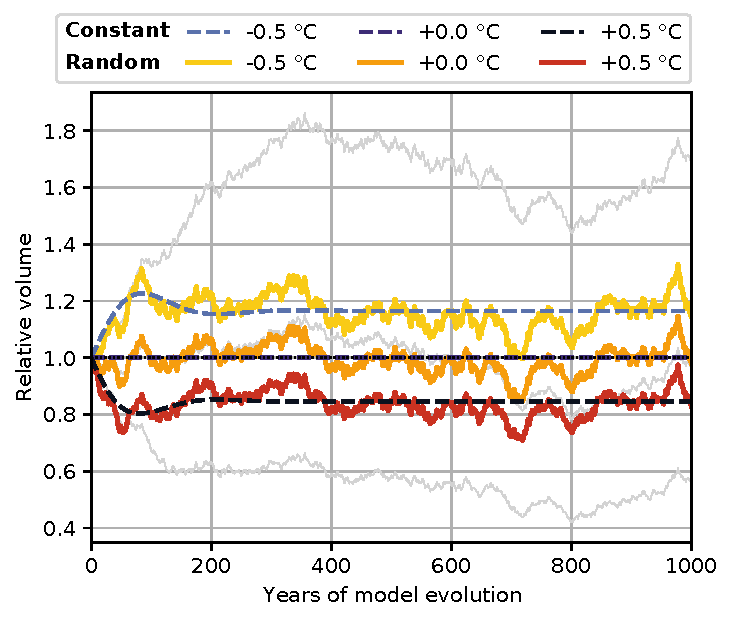
\includegraphics[width=\textwidth]{../plots/final_plots/time_series/single_glaciers/volume_norm_vas_Hintereisferner.pdf}
      \end{subfigure}
      \hfill
      % Flowline volume
      \begin{subfigure}[b]{0.476\textwidth}
        \caption{Flowline model, relative ice volume}
        \label{fig:hintereisferner:volume_fl}
        \centering
        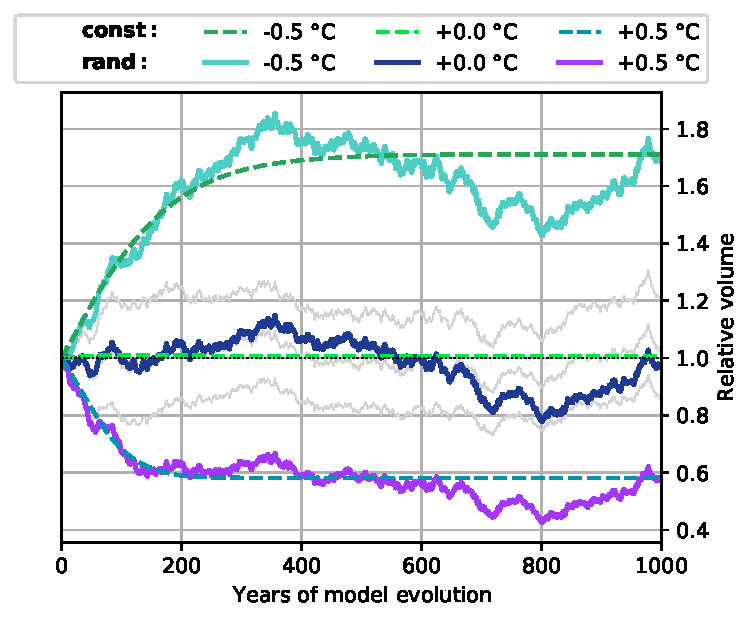
\includegraphics[width=\textwidth]{../plots/final_plots/time_series/single_glaciers/volume_norm_fl_Hintereisferner.pdf}
      \end{subfigure}

      % VAS area
      \begin{subfigure}[b]{0.476\textwidth}
        \caption{\Vas{} model, relative surface area}
        \label{fig:hintereisferner:area_vas}
        \centering
        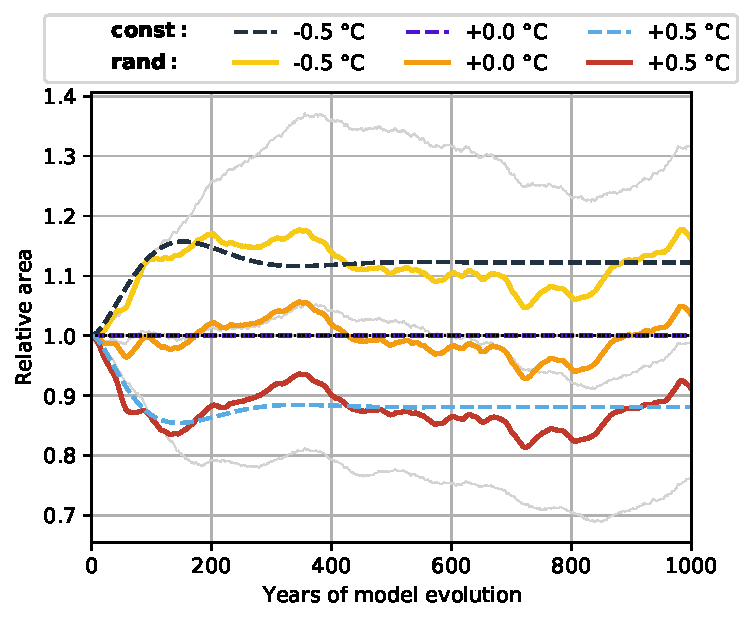
\includegraphics[width=\textwidth]{../plots/final_plots/time_series/single_glaciers/area_norm_vas_Hintereisferner.pdf}
      \end{subfigure}
      \hfill
      % Flowline area
      \begin{subfigure}[b]{0.476\textwidth}
        \caption{Flowline model, relative surface area}
        \label{fig:hintereisferner:area_fl}
        \centering
        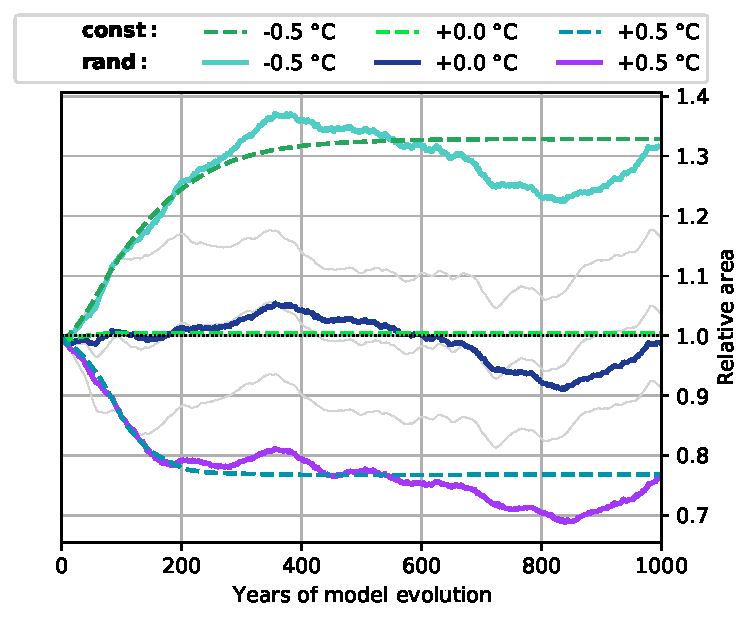
\includegraphics[width=\textwidth]{../plots/final_plots/time_series/single_glaciers/area_norm_fl_Hintereisferner.pdf}
      \end{subfigure}

      % VAS length
      \begin{subfigure}[b]{0.476\textwidth}
        \caption{\Vas{} model, relative glacier length}
        \label{fig:hintereisferner:length_vas}
        \centering
        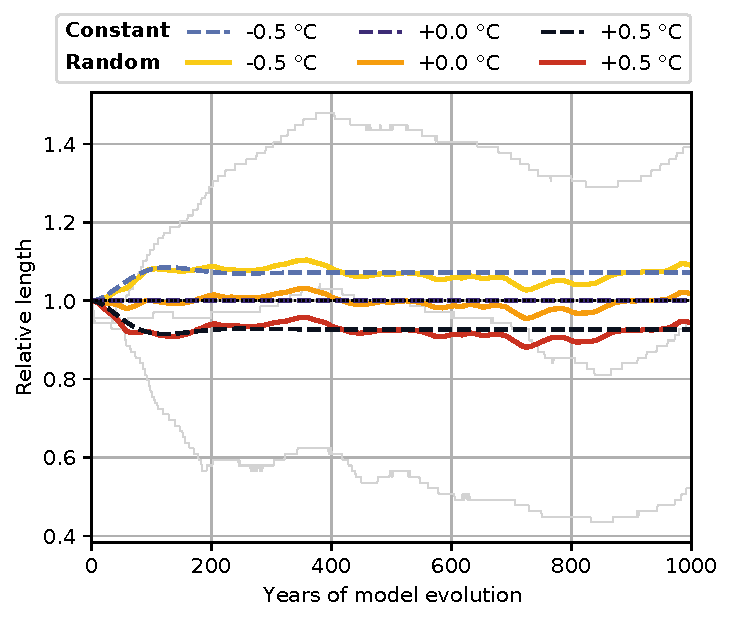
\includegraphics[width=\textwidth]{../plots/final_plots/time_series/single_glaciers/length_norm_vas_Hintereisferner.pdf}
      \end{subfigure}
      \hfill
      % Flowline length
      \begin{subfigure}[b]{0.476\textwidth}
        \caption{Flowline model, relative glacier length}
        \label{fig:hintereisferner:length_fl}
        \centering
        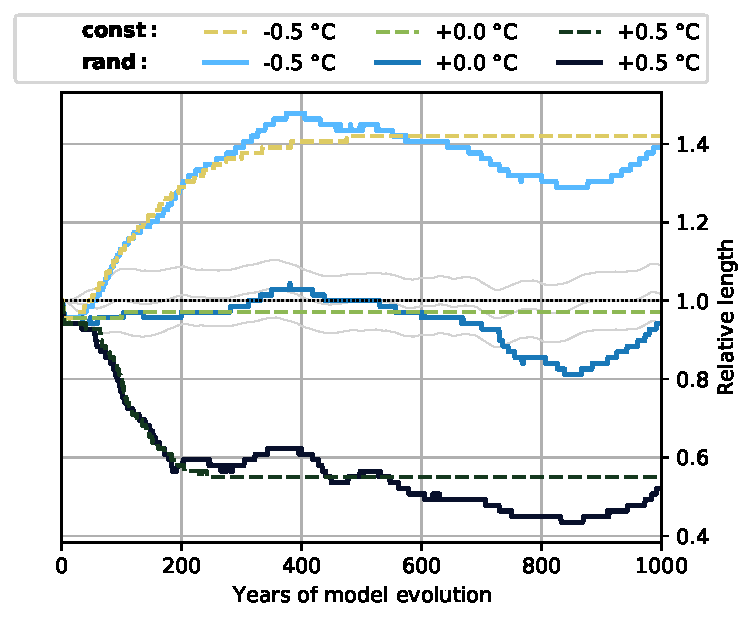
\includegraphics[width=\textwidth]{../plots/final_plots/time_series/single_glaciers/length_norm_fl_Hintereisferner.pdf}
      \end{subfigure}
      
      \caption{Temporal evolution of ice volume in (\subref{fig:hintereisferner:volume_vas}) and (\subref{fig:hintereisferner:volume_fl}), surface area in (\subref{fig:hintereisferner:area_vas}) and (\subref{fig:hintereisferner:area_fl}) and glacier length in (\subref{fig:hintereisferner:length_vas}) and (\subref{fig:hintereisferner:length_fl}) for Hintereisferner (RGI60-11.00897). The shown values area normalized with their respective initial values. The left panels show the result of the \vas{} model, the right panels show the results of the flowline model. Solid lines represent the random climate scenarios, while dashed lines represent the constant climate scenarios. All climate scenarios are based on an equilibrium climate. The applied temperature biases of \SI{-.5}{\celsius}, \SI{0}{\celsius} and \SI{+.5}{\celsius} are color coded, see legend for details. The dotted line indicates the initial volume. The light gray lines represent the volume evolutions of the other model, to facilitate comparisons.}
      \label{fig:hintereisferner}
    \end{figure}

  % section single_glacier_test_case_results (end)


  \section{Autocorrelation function and Power spectral density} % (fold)
  \label{sec:autocorrelation_and_power_spectral_density_results}
    
    % intro
    The autocorrelation function (ACF), partial autocorrelation function (PACF) and power spectral density (PSD) give insight into the periodicity and dominant frequencies of a given signal. Hereafter, the length signals of different model glaciers subjected to a constant climate with random year-to-year variabilities are used. The experiment is setup in analogy to the single glacier test case, since ACF, PACF and PSD should be performed on the time series of a single glacier. To avoid a N-of-1 experiment, five more individual glaciers are investigated, namely the Pasterze, Mer de Glace, Glacier d'Argentière, Aletschgletscher and Rhonegletscher. All glaciers are subjected to different random (white noise) climate conditions for 20\ 000 years. The spinup period during which the glaciers adjust to the different climate is clipped, with three different sizes of the same glacier. Hence, the temperature bias can be seen as label for glacier size rather than climate. For details about the experimental setup see Section~\ref{sub:autocorrelation_and_power_spectral_density_setup}. The ACF for lag times up to 200 years is shown in Figure~\ref{fig:acf}, the PACF for lag times up to 20 years in Figure~\ref{fig:pacf} and the PSD in Figure~\ref{fig:psd}. 

    \subsubsection{Autocorrelation function} % (fold)
    \label{ssub:autocorrelation_function_results}

      As a general observation over all glaciers and climate scenarios, the ACF shows high correlations for the first few lag times before decreasing exponentially. This points at an autoregressive (AR) term and a moving-average (MA) term in the data. An autoregressive-moving-average (ARMA) model predicts future values of a random variable based on a linear combination of past values and past error terms of said variable. This makes intuitive sense for glaciers, since the past and current glacier size and difference to the equilibrium value have a direct influence on next years glacier size. For example, the three-stage model of \citet{Roe2014} is an ARMA(3,3) model and performs well compared to a flowline model. However, let's look at the differences between \vas{} and flowline model first.

      The ACF of the \vas{} lengths are almost identical between different sizes of the same glacier, indicating that the glacier size has little to no effect on the transient behavior of the model. The \vas{} model represents a glacier as a simple cuboid, there is absolutely no information about the form of a glacier. The absolute dimesions of that cuboid seem to have less of an effect than other parameters. Some glaciers, like the Glacier d'Argentière, the Aletschgletscher and the Rhonegletscher show statistically significant negative correlations for higher lag terms between 100 and 300 years, while the others show very little to no significant negative correlation at all. However, no apparent relation between the strength of negative correlations for later lag times and any other glacier parameters, like the average slope or the model-internal lag times, was found. % TODO: hint on future work

      % AVG SLOPE
      % The average slope is one of the few additional geometric informations of the \vas{} model, even it is only implemented indirectly by the linear change of terminus elevation with glacier length. This slope is a glacier characteristic independent of its sizes and affects the temporal evolution. This can be seen in the ACF plots.  However, their is no pattern recognisable when compared with the average slope.
    
      The flowline model is able to represent different glacial geometries and grasp individual responses under different equilibrium climates, which can be seen in the vastly different ACFs. They differ from glacier to glacier, but also for different sizes of the same glacier. However, there are no discernible patterns, which again confirms the notion that the OGGM flowline model is capable of modeling each glacier's individual response. The following list points to some particular observations:
      \begin{itemize}
        \item for Hintereisferner the ACFs of the flowline model are stronger than those of the \vas{} model, while for Mer de Glace and Großer Aletschgletscher they are lower (for all tested climate scenarios, i.e., all different sizes)
        \item the flowline model of the Pasterze shows a strong autocorrelation under the equilibrium climate, i.e., for its medium size, (>0.7 for lags times between 0 and 95 years, still >0.43 for 200 years lag time, statistically significant up until a lag time of 232 years), while under a warmer and colder equilibrium climate (\SI{\pm0.5}{\celsius}) the autocorrelation of all lag times is lower than for the \vas{} model
        \item similarly, the flowline model of the Glacier d'Argentière shows a strong autocorrelation under the warmer equilibrium climate (\SI{+0.5}{\celsius}), while the autocorrelation under the other two climate scenarios is even lower than the ACF of the \vas{} model
      \end{itemize}
      The only observation made for all glaciers, it that the \vas{} model shows a stronger autocorrelation for shorter lag time (i.e., less than about 20 years) than the flowline model. This is true even for glaciers, where the autocorrelation of the flowline mode is generally stronger than for the \vas{} model (e.g., Hintereisferner).

      Strong correlations for short lag times influence all following lag terms. For example, an exponentially decaying signal which halves its value with each time step $\Phi(t) = 0.5 \Phi(t-1)$ will have an autocorrelation of 0.5 for lag 1, 0.25 for lag 2, 0.125 for lag 3, and so on. Depending on the sample size these values will be statistically significant, even though only one lag term is included in the definition of the signal (i.e., AR(1) process). The partial autocorrelation function (PACF) measures only these direct influences, eliminating the effects of all shorter lag times. All the PACFs of the \vas{} model lengths show a strong positive correlation for lag times of 1 year, followed by a strong negative correlation which then decreases slowly towards zero. Correlations for lag times 10 and greater are not or only marginally significant. Again, no discernable differences between different sizes of the same glacier and very little differences from one glacier to another. The PACFs for the flowline model lengths show a high correlation for lag time of 1 year, before decreasing towards zero. The decrease towards statistical insignificant correlations happens faster for some glaciers (e.g., only lag 1 and 2 show a significant correlation for the Pasterze and the Aletschgletscher under the warmer equilibirum) and slower for others (e.g., the Rhonegletscher shows significant correlations for lag times up to 5 and 6 years, depending on the temperature bias). Hereby, there are differences in PACFs between different sizes of the same glacier. For higher lag times between 10 and 20 years there are some negative correlations, even if only marginally significant.

      The number of statistically significant terms of the PACF informs on the order $p$ of the AR(p) model. The order specifies the number lag terms are considered. Analogously, the order $q$ of the MA(q) model can be estimated from the number of significant terms of the ACF. By this definition, the \vas{} and flowline model length could be modeled with an ARMA(11,103) and ARMA(5,150) model, respectively. Hereby, the orders are taken as average over all glaciers and climate scenarios. While an AR model with 11 lag terms is big but still feasable, a MA model with over 100 lag terms is neither practicable nor does it make sense. Especially, since \citet{Roe2014} use an ARMA(3,3) model to produce comparable results to a flowline model.

      It is not the intent of this work to investigate the relation between a glacier's geometry and its ACF, neither to fit an ARMA model to the data. Hence, this qualitative first look has to suffice. However, it is most notable that the OGGM flowline model behaves differently not only for different glaciers, but also for different sizes of the same glacier. The \textit{one size fits all} approach of the \vas{} model produces more homogenous results, the ACFs and PACFs are mostly independent of a glacier's size.

      \begin{figure}[htp]
        \centering
        
        \begin{subfigure}[b]{0.48\textwidth}
          \caption{RGI60-11.00897 - Hintereisferner}
          \label{fig:acf:hintereisferner}
          \centering
          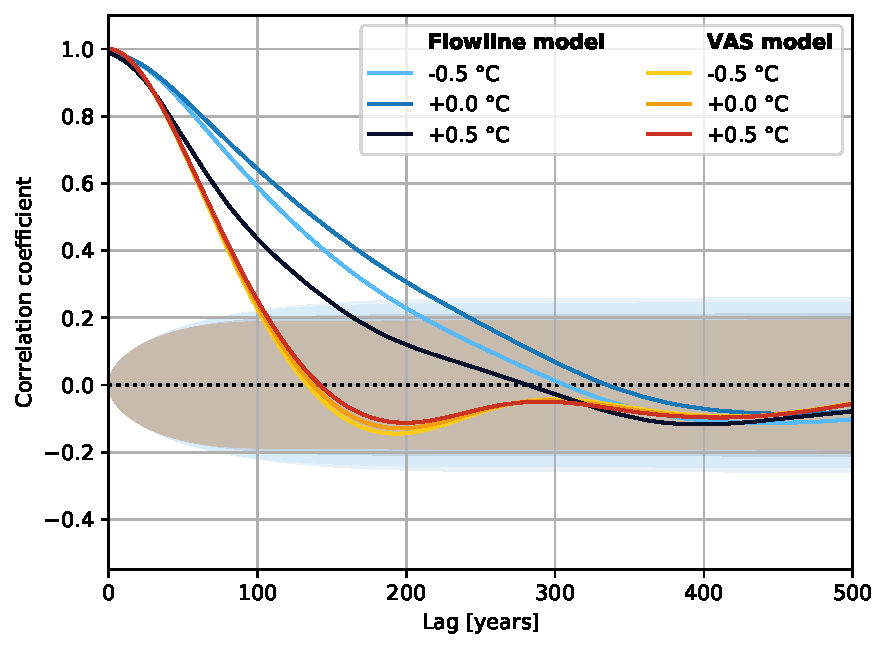
\includegraphics[width=\textwidth]{../plots/final_plots/acf/Hintereisferner.pdf}
        \end{subfigure}
        \hfill
        \begin{subfigure}[b]{0.48\textwidth}
          \caption{RGI60-11.00106 - Pasterze}
          \label{fig:acf:pasterze}
          \centering
          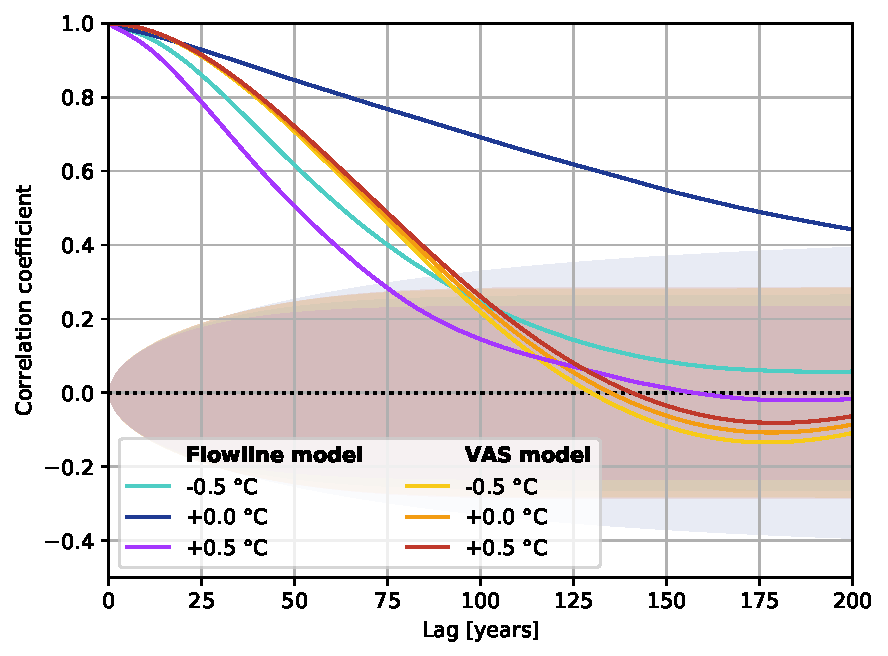
\includegraphics[width=\textwidth]{../plots/final_plots/acf/Pasterze.pdf}
        \end{subfigure}

        \begin{subfigure}[b]{0.48\textwidth}
          \caption{RGI60-11.03643 - Mer de Glace}
          \label{fig:acf:mer_de_glace}
          \centering
          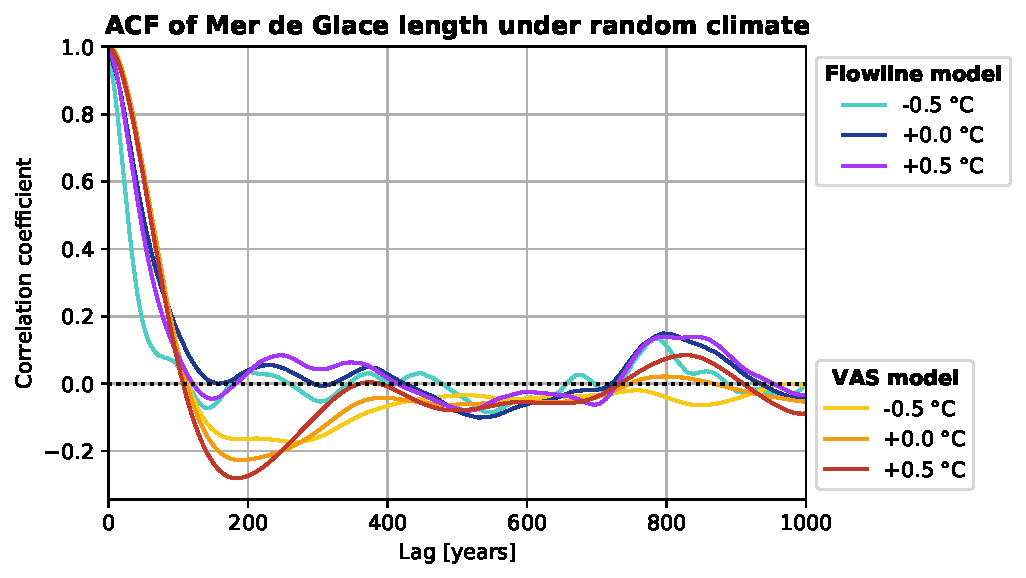
\includegraphics[width=\textwidth]{../plots/final_plots/acf/Mer_de_Glace.pdf}
        \end{subfigure}
        \hfill
        \begin{subfigure}[b]{0.48\textwidth}
          \caption{RGI60-11.03638 - d'Argentière}
          \label{fig:acf:glacier_d_argentiere}
          \centering
          \includegraphics[width=\textwidth]{../plots/final_plots/acf/Glacier_d'Argentière.pdf}
        \end{subfigure}

        \begin{subfigure}[b]{0.48\textwidth}
          \caption{RGI60-11.01450 - Großer Aletschgletscher}
          \label{fig:acf:großer_aletschgletscher}
          \centering
          \includegraphics[width=\textwidth]{../plots/final_plots/acf/Großer_Aletschgletscher.pdf}
        \end{subfigure}
        \hfill
        \begin{subfigure}[b]{0.48\textwidth}
          \caption{RGI60-11.01238 - Rhonegletscher}
          \label{fig:acf:rhonegletscher}
          \centering
          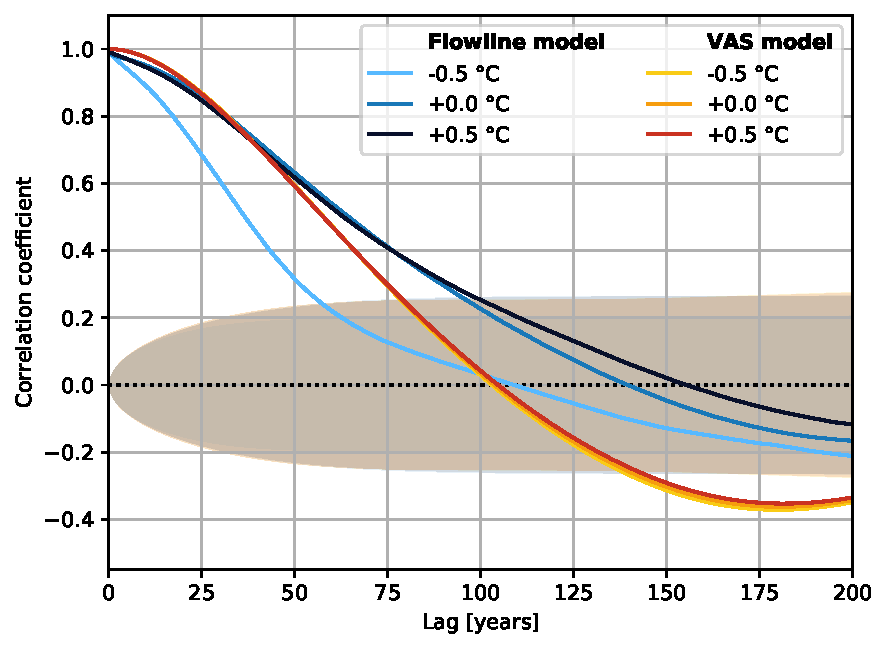
\includegraphics[width=\textwidth]{../plots/final_plots/acf/Rhonegletscher.pdf}
        \end{subfigure}

        \caption{Autocorrelation function of modeled length for lag times between zero and 200 years. Different lines represent different combinations of evolution model and climate scenario.
        The random climate scenario is based on an equilibrium climate, with different temperature biases.
        Cyan, blue and purple lines represent the flowline model, while yellow, orange and red lines represent the \vas{} model, with a temperature bias of \SI{-.5}{\celsius}, \SI{0}{\celsius} and \SI{+.5}{\celsius}, respectively.
        The \SI{99}{\percent} confidence intervals are shaded in the corresponding colors.}
        \label{fig:acf}
      \end{figure}

      \begin{figure}[htp]
        \centering
        
        \begin{subfigure}[b]{0.48\textwidth}
          \caption{RGI60-11.00897 - Hintereisferner}
          \label{fig:pacf:hintereisferner}
          \centering
          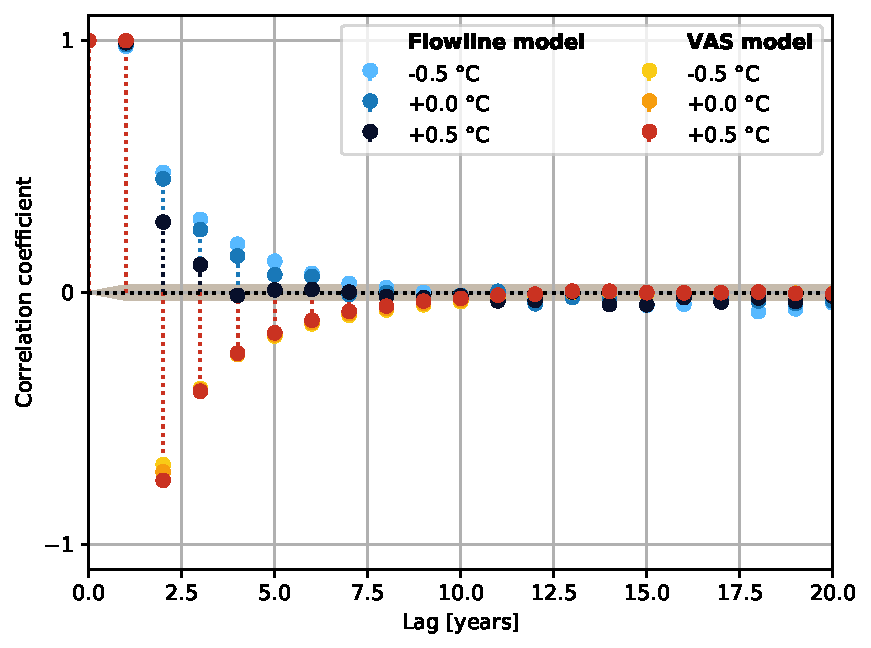
\includegraphics[width=\textwidth]{../plots/final_plots/pacf/Hintereisferner.pdf}
        \end{subfigure}
        \hfill
        \begin{subfigure}[b]{0.48\textwidth}
          \caption{RGI60-11.00106 - Pasterze}
          \label{fig:pacf:pasterze}
          \centering
          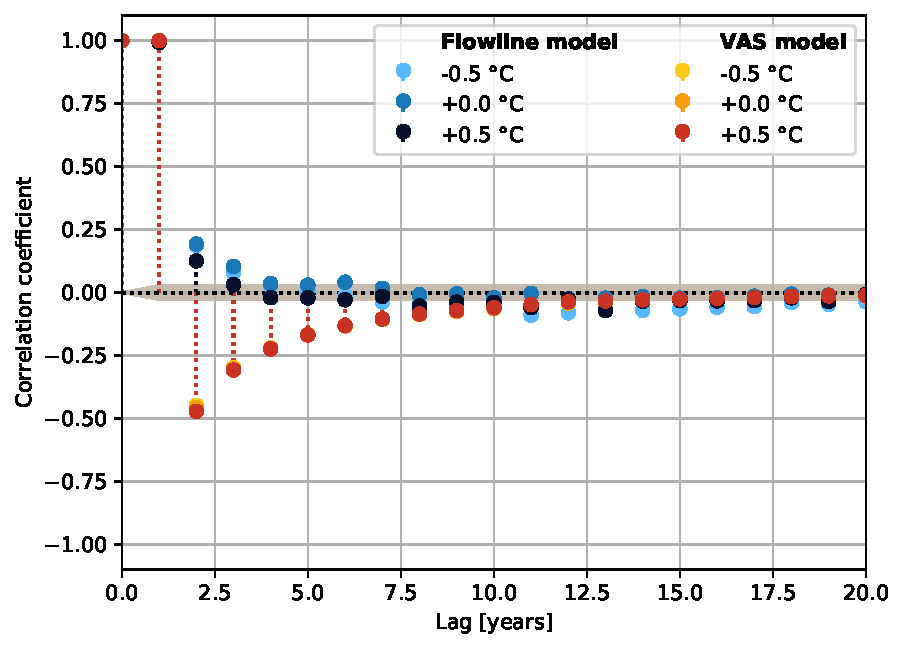
\includegraphics[width=\textwidth]{../plots/final_plots/pacf/Pasterze.pdf}
        \end{subfigure}

        \begin{subfigure}[b]{0.48\textwidth}
          \caption{RGI60-11.03643 - Mer de Glace}
          \label{fig:pacf:mer_de_glace}
          \centering
          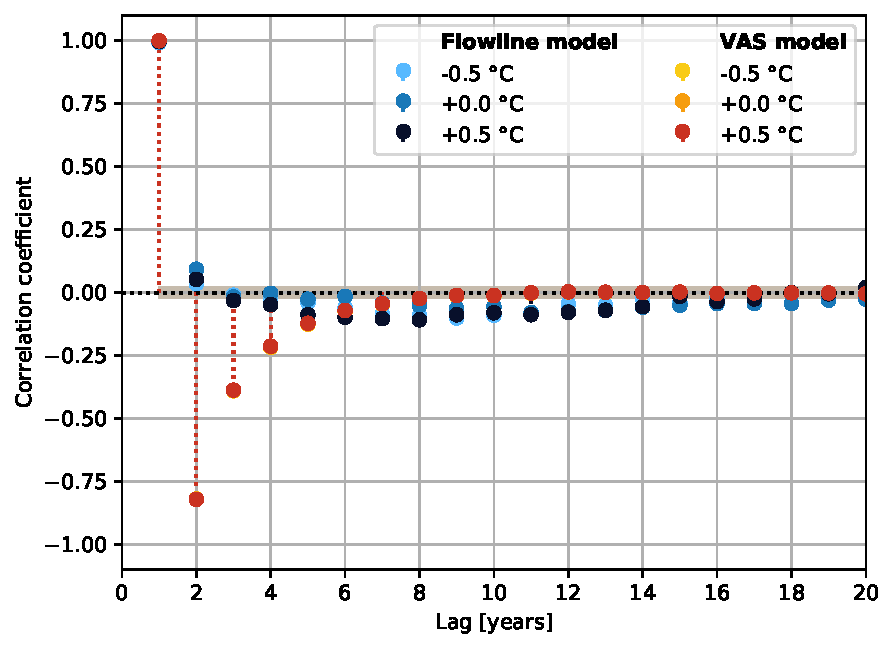
\includegraphics[width=\textwidth]{../plots/final_plots/pacf/Mer_de_Glace.pdf}
        \end{subfigure}
        \hfill
        \begin{subfigure}[b]{0.48\textwidth}
          \caption{RGI60-11.03638 - d'Argentière}
          \label{fig:pacf:glacier_d_argentiere}
          \centering
          \includegraphics[width=\textwidth]{../plots/final_plots/pacf/Glacier_d'Argentière.pdf}
        \end{subfigure}

        \begin{subfigure}[b]{0.48\textwidth}
          \caption{RGI60-11.01450 - Großer Aletschgletscher}
          \label{fig:pacf:großer_aletschgletscher}
          \centering
          \includegraphics[width=\textwidth]{../plots/final_plots/pacf/Großer_Aletschgletscher.pdf}
        \end{subfigure}
        \hfill
        \begin{subfigure}[b]{0.48\textwidth}
          \caption{RGI60-11.01238 - Rhonegletscher}
          \label{fig:pacf:rhonegletscher}
          \centering
          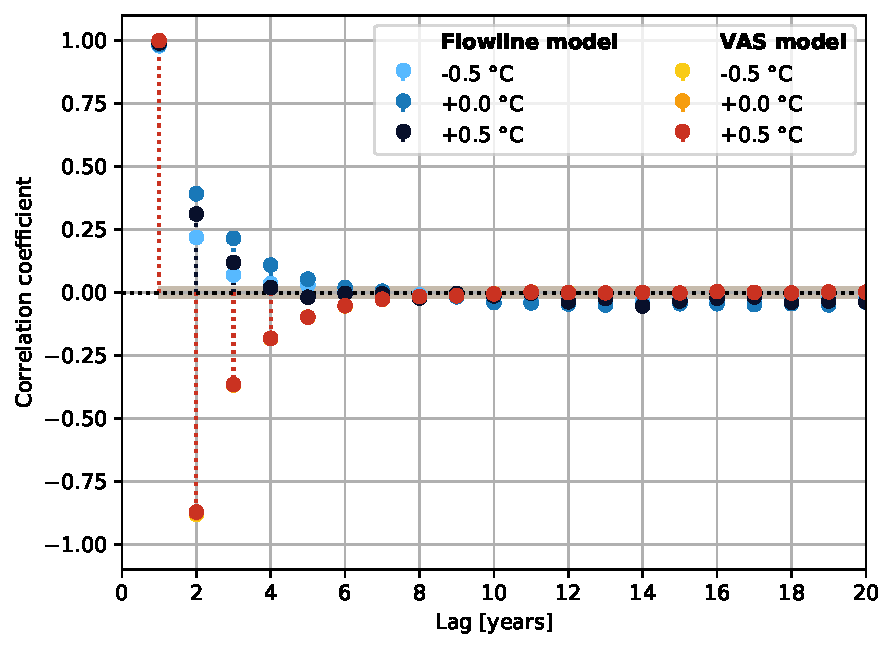
\includegraphics[width=\textwidth]{../plots/final_plots/pacf/Rhonegletscher.pdf}
        \end{subfigure}

        \caption{Partial autocorrelation function of modeled length for lag times between zero and 200 years. Different lines represent different combinations of evolution model and climate scenario.
        The random climate scenario is based on an equilibrium climate, with different temperature biases.
        Cyan, blue and purple lines represent the flowline model, while yellow, orange and red lines represent the \vas{} model, with a temperature bias of \SI{-.5}{\celsius}, \SI{0}{\celsius} and \SI{+.5}{\celsius}, respectively.
        The \SI{99}{\percent} confidence intervals are shaded in the corresponding colors.}
        \label{fig:pacf}
      \end{figure}

    % subsubsection autocorrelation_function_results (end)

    \subsubsection{Power spectral density} % (fold)
    \label{ssub:power_spectral_density_results}
    
      % intro
      The power spectral density is estimated via Welch's method. Welch's method reduces the variance in the estimated power density by time-averaging, at the cost of frequency resolution (e.g., TODO: citation). As for the autocorrelation analysis, the initial 1000 years of the adjustment period are clipped. The resulting 9000 data points are divided into nine time windows with a window size of 1800 datapoints and a \SI{50}{\percent} overlap. The windows are tapered using the Hann function. For details about additional parameters see the default values of the python function \href{https://docs.scipy.org/doc/scipy/reference/generated/scipy.signal.welch.html}{\lstinline`scipy.signal.welch`}. The power spectral density should not be computed from the aggragate glacier length of all Alpine glaciers, since mirroring oscillations would cancel each other out. In order to avoid a n-of-1 experiment, the follwing six Alpine glaciers are shown below %TODO Showcase glaciers.

      % general
      For all glaciers and all cliamte scenarios, the power density of the length change signal decreases with increasing frequency. This makes intuituve sense, since changes in glacier length are mainly driven by long term climatic trends and less by inter-annual variabilities in the climatic forcing. Glaciers are low-pass filters

      As seen before, the flowline model glaciers react stronge to given changes in climate than the VAS model glaciers. This is reflected in an overall higher power density (approximately one order of magnitude) of the flowline model runs.

      The flowline model runs are good examples of low pass filter. A low pass filter passes lower frequencies while attenuating (or rejecting) higher frequencies. And so does the glacier (model). For frequencies up to 

      After an initial decrease in power density with increasing frequency, the power density stays fairly constant for periods in the order of magnitue of ten years. The longterm changes of the climate system are driving the glacial evolution, while the short term changes in monthly or yearly climatic parameters have little to no effect. The power spectral density anlysis suggests that trends  shorter than 10 years (corresponding to a frequency of 0.1 year$^{-1}$) are filtered by the flowline model.

      The power spectral density curves of the \vas{} show no discernible differences between the different temperature biases and are even comparable across different glaciers. In fact, the maximum relative difference from one curve to another is \SI{150}{\percent}

      Similar to the time series and the auto correlation analysis, the power spectral density of \vas{} model’s length change signal does not change for different temperature biases. Even the differences between glaciers is 

      The PSD of the VAS model is almost identical between runs with different temperature biases, attributed to the linear (and symmetric) behaviour seen before. The flowline model produces a less coherent PSD between the runs with different temperature bias, whereby the equilibrium run and the positive mass balance run are more alike.

      % vas vs flowline

      \begin{figure}[htp]
        \centering
        \begin{subfigure}[b]{0.48\textwidth}
          \caption{RGI60-11.00897 - Hintereisferner}
          \label{fig:psd:hintereisferner}
          \centering
          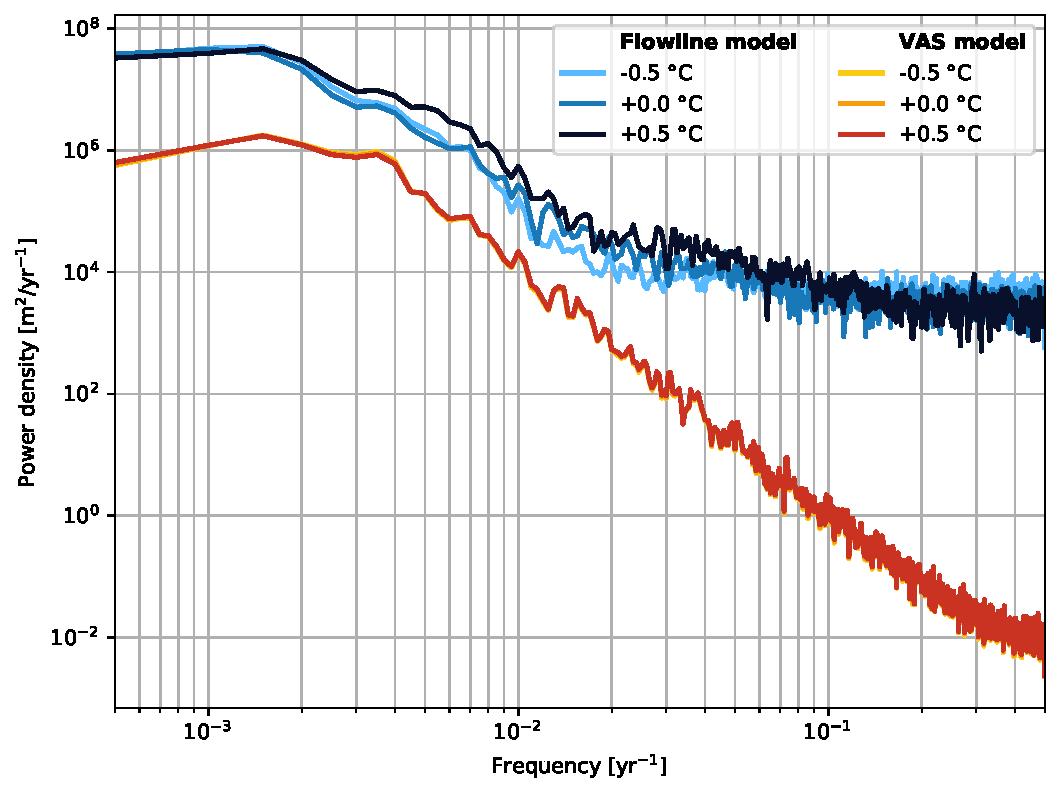
\includegraphics[width=\textwidth]{../plots/final_plots/psd/Hintereisferner.pdf}
        \end{subfigure}
        \hfill
        \begin{subfigure}[b]{0.48\textwidth}
          \caption{RGI60-11.00106 - Pasterze}
          \label{fig:psd:pasterze}
          \centering
          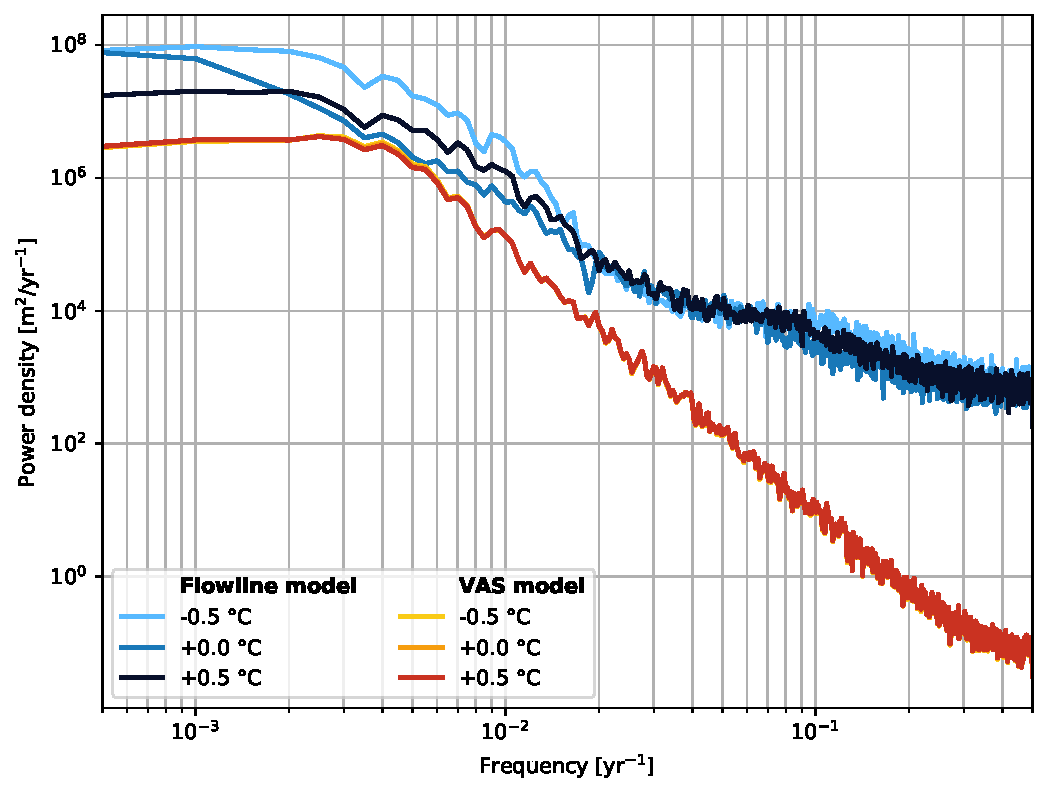
\includegraphics[width=\textwidth]{../plots/final_plots/psd/Pasterze.pdf}
        \end{subfigure}
        \begin{subfigure}[b]{0.48\textwidth}
          \caption{RGI60-11.03643 - Mer de Glace}
          \label{fig:psd:mer_de_glace}
          \centering
          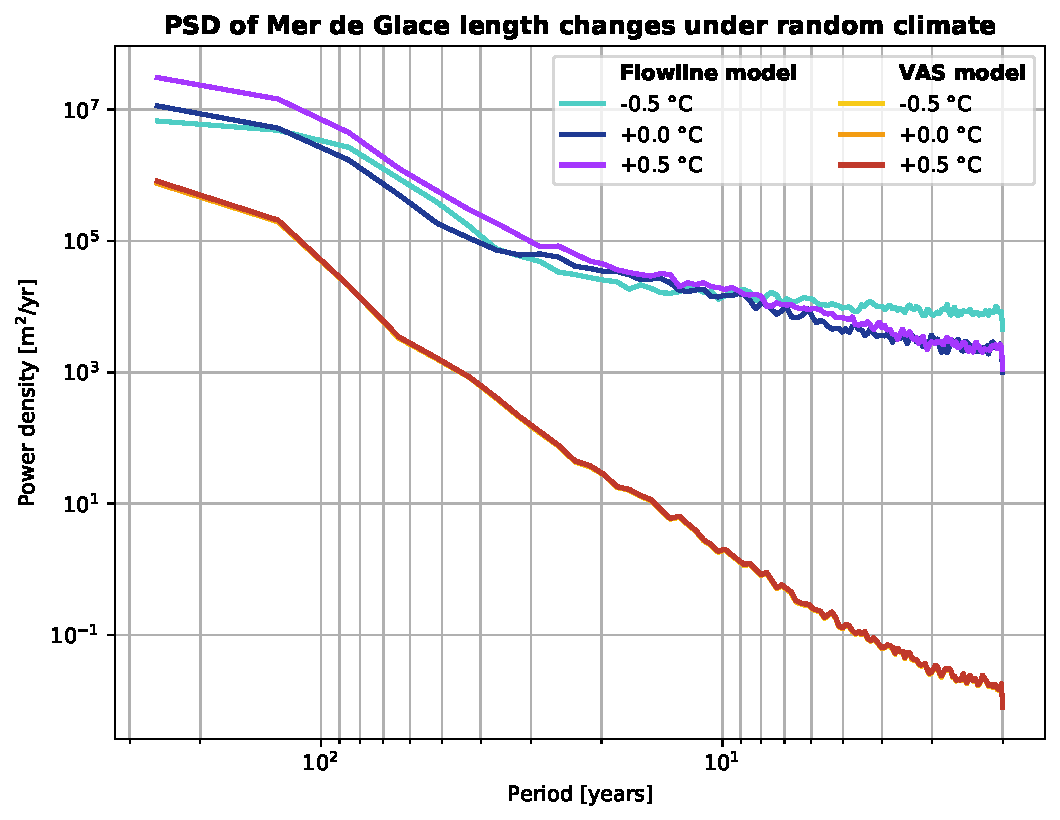
\includegraphics[width=\textwidth]{../plots/final_plots/psd/Mer_de_Glace.pdf}
        \end{subfigure}
        \hfill
        \begin{subfigure}[b]{0.48\textwidth}
          \caption{RGI60-11.03638 - d'Argentière}
          \label{fig:psd:glacier_d_argentiere}
          \centering
          \includegraphics[width=\textwidth]{../plots/final_plots/psd/Glacier_d'Argentière.pdf}
        \end{subfigure}
        \begin{subfigure}[b]{0.48\textwidth}
          \caption{RGI60-11.01450 - Großer Aletschgletscher}
          \label{fig:psd:großer_aletschgletscher}
          \centering
          \includegraphics[width=\textwidth]{../plots/final_plots/psd/Großer_Aletschgletscher.pdf}
        \end{subfigure}
        \hfill
        \begin{subfigure}[b]{0.48\textwidth}
          \caption{RGI60-11.01238 - Rhonegletscher}
          \label{fig:psd:rhonegletscher}
          \centering
          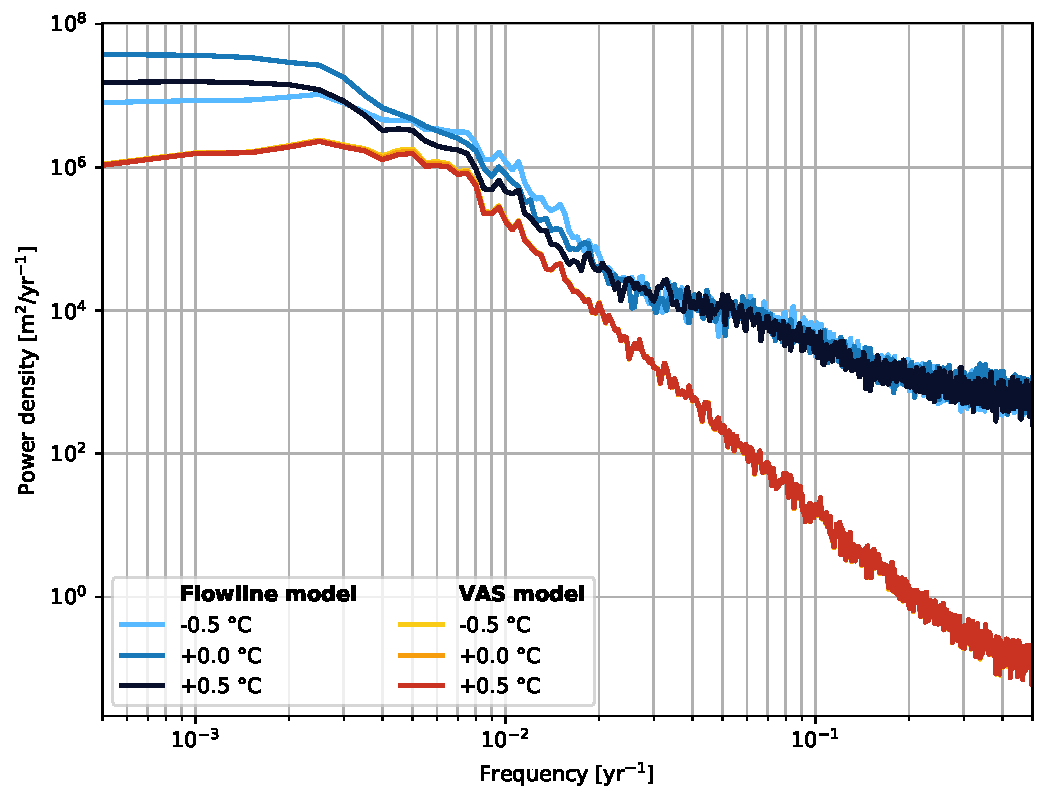
\includegraphics[width=\textwidth]{../plots/final_plots/psd/Rhonegletscher.pdf}
        \end{subfigure}

        \caption{Power spectral density of modeled glacier length for different alpine glaciers. Different lines represent different combinations of evolution models and climate scenarios. The climate scenarios are based on a randomized equilibrium climate, with different temperature biases. Cyan, blue and purple lines represent the flowline model, while yellow, orange and red lines represent the \vas{} model, with a temperature bias of \SI{-.5}{\celsius}, \SI{0}{\celsius} and \SI{+.5}{\celsius}, respectively. Note the differences in y-axis scales.}
        \label{fig:psd}
      \end{figure}
    
    % subsubsection power_spectral_density_results (end)

  % section autocorrelation_fand_power_spectral_density_results (end)

  \section{Regional runs with all Alpine glaciers} % (fold)
  \label{sec:regional_runs_with_all_alpine_glaciers_results}

    \Vas{} should not be applied to individual glaciers but to populations of glaciers \citep{Bahr2015}. This is were the scaling approach shows its strength. The law of large number assures a reasonable estimation of the collective glacier ice volume, since random errors will be canceled out by each other. This section compares the behavior of \vas{} model applied to all Alpine glaciers with differnte climate scenarios to the OGGM flowline model, as was done above for a single glacier (see Section~\ref{sec:single_glacier_test_case_results}).
    In contrast to the single glacier test case, the \vas{} model and the flowline model each use their respective \tstar{} reference table. Additionally, a possible mass balance residual \bias{} is applied. This ensure to produce results as physical as possible. Again, both mass balance models simulate different climates with the same three temperature biases as above, based on the equilibirum period centered around \lstinline`y0` = \tstar{}. For more details about the experimenta setup see Section~\ref{sub:regional_runs_with_all_alpine_glaciers_setup}. The time series plots of normalized and absolute volume are shown in Figure~\ref{fig:histalp_commitment}.

    Both evolution models run for 1000 years with the \lstinline`ConstantMassBalance` model and the \lstinline`RandomMassBalance` model. A random climate with its year-to-year fluctuations is obviously more physical than a completely constant climate. However, the resulting changes in glacier ice volume under both climate scenarios are almost identical. Over the last 200 years of the simulations, the differences in aggragate ice volumes between the constant and random climate scenario average around \SI{0.6}{\percent} to \SI{0.7}{\percent} for the \vas{} model and \SI{0.7}{\percent} to \SI{2.3}{\percent} for the flowline model, depending on the temperature bias (see \ref{fig:histalp_commitment}). % hef_histalp_commitment.ipynb
    This makes intuitive sense, considering that glaciers act as natural low-pass filters for climatic variabilities. Short time climatic variability has little to no effect on a glacier's ice volume, and especially not on the aggregate ice volume of an entire region. Therefore, the following discussion is simplified by only considering the constant climate scenarios.

    The \vas{} model estimates a total Alpine ice volume of \SI{139}{\cubic\kilo\meter} (\SI{+6}{\percent}), \SI{115}{\cubic\kilo\meter} (\SI{-12}{\percent}) and \SI{95}{\cubic\kilo\meter} (\SI{-27}{\percent}), while the flowline model estimates a total Alpine ice volume of \SI{236}{\cubic\kilo\meter} (\SI{+45}{\percent}), \SI{147}{\cubic\kilo\meter} (\SI{-10}{\percent}) and \SI{86}{\cubic\kilo\meter} (\SI{-47}{\percent}), for a temperature bias of \SI{-.5}{\celsius}, \SI{0}{\celsius} and \SI{+.5}{\celsius}, respectively. 
    Both evolution models adjust their initial ice volume downwards under equilibrium climate. This can be explained by the mass balance residual \bias{} and indicates that either
    \begin{enumerate*}[label=(\alph*)]
      \item the 2003 RGI geometries are not sustainable by any 31-period in the HISTALP records or
      \item the 2003 RGI glaciers are in a transient state and still retracting even after the climate is held constant
    \end{enumerate*}
    \citep{Maussion2019}.
    This sag could be eliminated by a spin-up period, but since the absolute values are of less interest for now it seems unnecessary. Besides that, all characteristics of the \vas{} model found for the Hintereisferner test case can be seen here as well. The \vas{} scaling model underestimates the changes in ice volume, produces symmetric results and adjusts faster to a given step change in climate. %ASK#2 compute regional time scales?!
    Even the oscillatory behavior is still found on the regional scale.
    All in all, the \vas{} model does a bad job if we consider the flowline model results as the reality. However, 
    The next section explores the possibility of tuning the \vas{} model via different parameters of the used scaling realtions. This also provides a range of possible results and serves as uncertainty estimation.

    \begin{figure}[htp]
      \centering
      \begin{subfigure}[b]{0.48\textwidth}
        \caption{\Vas{} model, relative glacier volume}
        \label{fig:histalp_commitment:volume_norm_const}
        \centering
        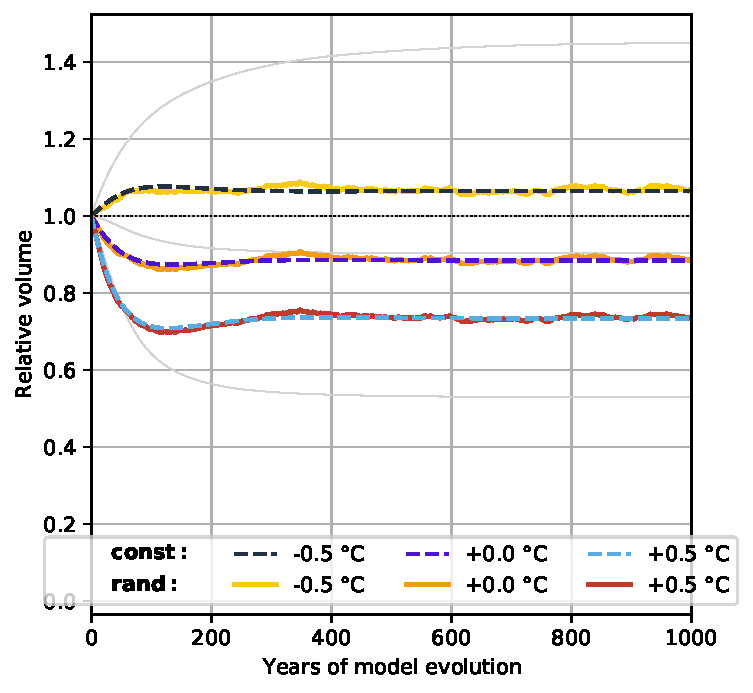
\includegraphics[width=\textwidth]{../plots/final_plots/time_series/histalp_commitment/volume_norm_vas.pdf}
      \end{subfigure}
      \hfill
      \begin{subfigure}[b]{0.48\textwidth}
        \caption{Flowline model, relative glacier volume}
        \label{fig:histalp_commitment:volume_norm_random}
        \centering
        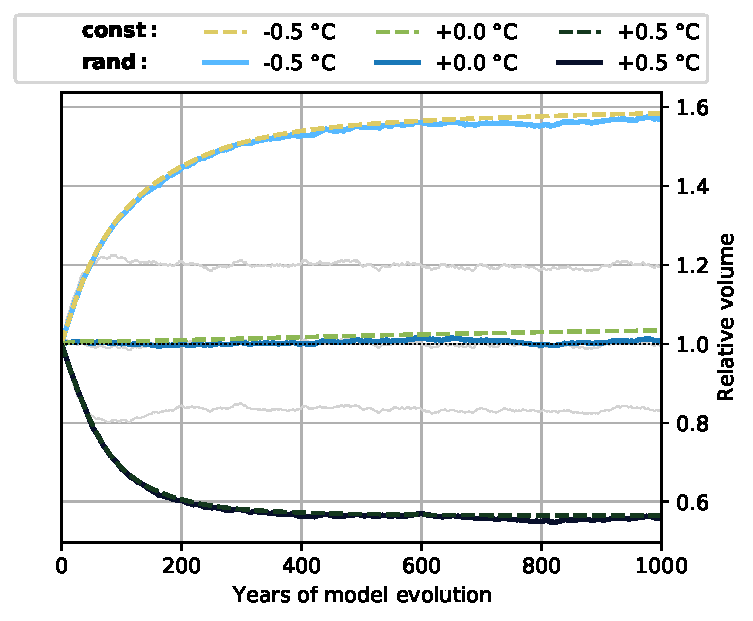
\includegraphics[width=\textwidth]{../plots/final_plots/time_series/histalp_commitment/volume_norm_fl.pdf}
      \end{subfigure}
      \begin{subfigure}[b]{0.48\textwidth}
        \caption{\Vas{} model, absolute glacier volume}
        \label{fig:histalp_commitment:volume_abs_const}
        \centering
        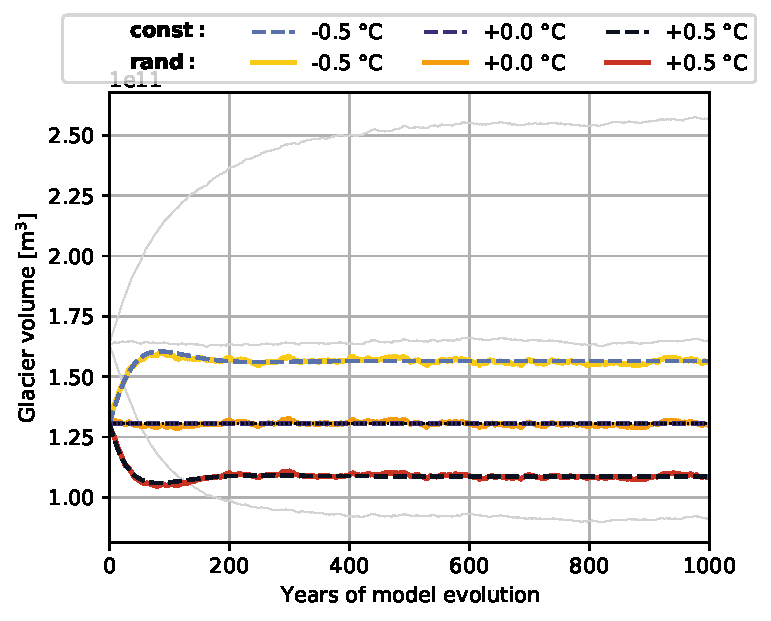
\includegraphics[width=\textwidth]{../plots/final_plots/time_series/histalp_commitment/volume_abs_vas.pdf}
      \end{subfigure}
      \hfill
      \begin{subfigure}[b]{0.48\textwidth}
        \caption{Flowline model, absolute glacier volume}
        \label{fig:histalp_commitment:volume_abs_random}
        \centering
        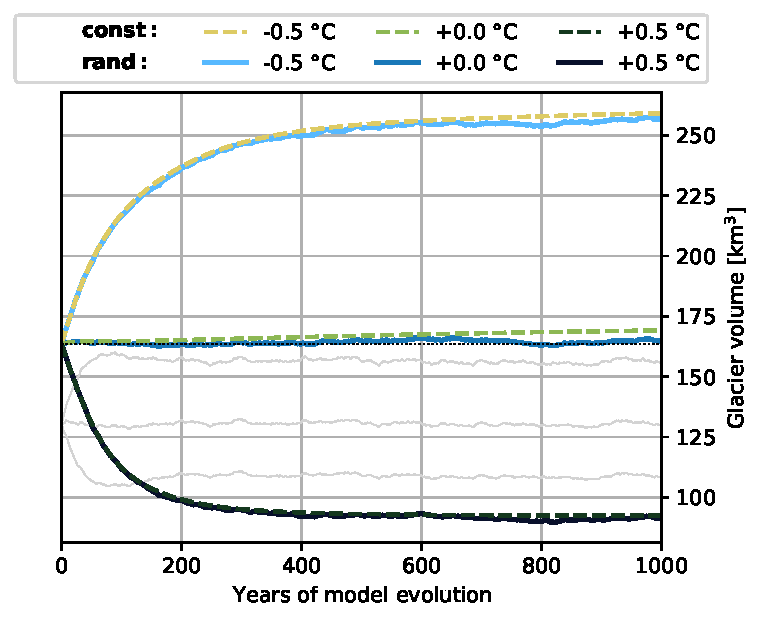
\includegraphics[width=\textwidth]{../plots/final_plots/time_series/histalp_commitment/volume_abs_fl.pdf}
      \end{subfigure}
      
      \caption{Time series of total ice volume for all glaciers in the HISTALP domain. The upper two panels show the relative glacier ice volume, normalized with the initial values, while the lower two panels show the absolute glacier ice volume. The left panels show the result of the \vas{} model, the right panels show the results of the flowline model. Solid lines represent the random climate scenarios, while dashed lines represent the constant climate scenarios. All climate scenarios are based on an equilibrium climate, with one of three different temperature biases.
      Yellow, orange and red solid lines represent the \vas{} model, while cyan, blue and purple solid lines represent the flowline model, under a random climate with a temperature bias of \SI{-.5}{\celsius}, \SI{0}{\celsius} and \SI{+.5}{\celsius}, respectively. Yellow, orange and red dashed lines represent the \vas{} model, while cyan, blue and purple dashed lines represent the flowline model, under a constant climate with a temperature bias of \SI{-.5}{\celsius}, \SI{0}{\celsius} and \SI{+.5}{\celsius}, respectively. %TODO change colors
      The dotted line indicate the initial volume. The light gray lines represent the volume evolutions of the other model, to facilitate comparisons.}
      \label{fig:histalp_commitment}
    \end{figure}

  % section regional_runs_with_all_alpine_glaciers_results (end)

  \section{Sensitivity experiments} % (fold)
  \label{sec:sensitivity_experiments_results}

    All the experiments performed above show quite large differences in projected ice volume change between the \vas{} model and the flowline model. However, the ``out-of-the-box'' scaling model is maybe not the best fit for the Alps and it is definitely not a good fit for any single glacier. Hence, a set of tuning parameters may improve the model performance.
    The most obvious tuning parameters are the model-internal time scales and the scaling constants and scaling exponents. The following sensitivity experiments run the \vas{} model with different values for these parameters. Experiments are perforemd on the Hintereisferner (RGI60-11.00897) and the all Alpine glaciers in the HISTALP domain, in each case with a constant equilibrium climate scenario and a positive temperature bias of \SI{+0.5}{\celsius}. For details about the experimental setup see Section~\ref{sub:sensitivity_experiments_setup}.

    \begin{tldrbox}[Sensitivity experiments]{tldr:sensitivity_experiments_results}
      \item the model-internal time scales control the damping ratio of the oscillation, longer time scales correspond to stronger overshoots
      \item halving the model-internal time scales leads to an asymptotical change in aggregte ice volume of the HISTALP domain, without any oscillations
      \item different scaling constants lead to a different initial ice volume and a different initial glacier length, which in turn affect the e-folding time scales
      \item changing the scaling constants has little to no effect on the normalized volume change and normalized equilibrium volume
      \item custom scaling constants and exponents increase the change in ice volume ever so slightly, but the results are still not comparable to the flowline model
    \end{tldrbox}
    
    \begin{figure}[ht]
      \centering
      % HEF time scales
      \begin{subfigure}[b]{0.476\textwidth}
        \caption{Hintereisferner, different model-internal time scales}
        \label{fig:sensitivity:time_scales_hef}
        \centering
        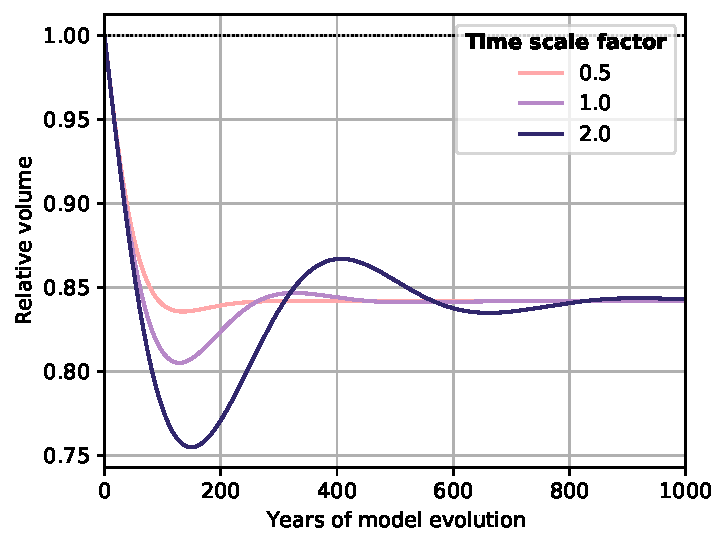
\includegraphics[width=\textwidth]{../plots/final_plots/sensitivity/time_scales_hef.pdf}
      \end{subfigure}
      \hfill
      % HEF scaling params
      \begin{subfigure}[b]{0.476\textwidth}
        \caption{Hintereisferner, different scaling constants}
        \label{fig:sensitivity:scaling_params_hef}
        \centering
        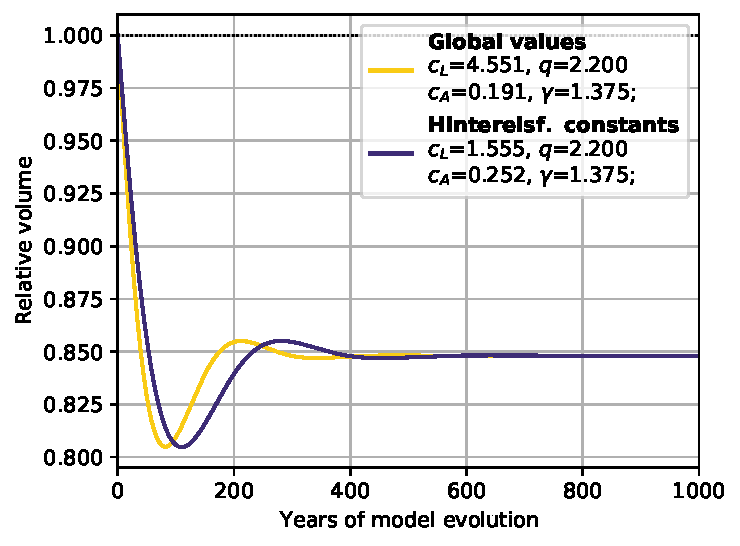
\includegraphics[width=\textwidth]{../plots/final_plots/sensitivity/scaling_params_hef.pdf}
      \end{subfigure}
      
      % HISTALP time scales
      \begin{subfigure}[b]{0.476\textwidth}
        \caption{HISTALP domain, different model-internal time scales}
        \label{fig:sensitivity:time_scales_histalp}
        \centering
        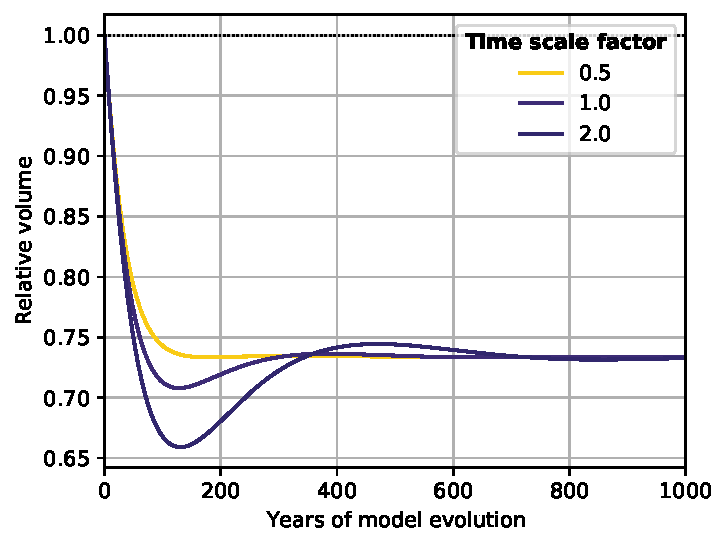
\includegraphics[width=\textwidth]{../plots/final_plots/sensitivity/time_scales_histalp.pdf}
      \end{subfigure}
      \hfill
      % HISTALP scaling params
      \begin{subfigure}[b]{0.476\textwidth}
        \caption{HISTALP domain, different scaling constants and scaling exponents}
        \label{fig:sensitivity:scaling_params_histalp}
        \centering
        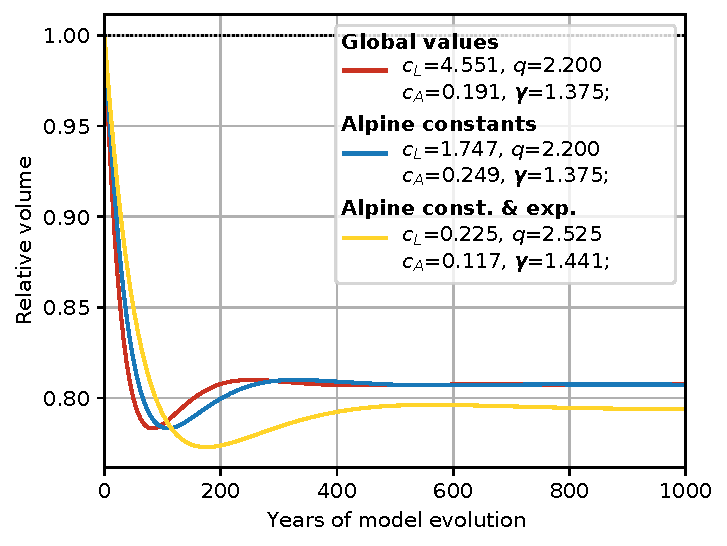
\includegraphics[width=\textwidth]{../plots/final_plots/sensitivity/scaling_params_histalp.pdf}
      \end{subfigure}
      
      \caption{Temporal evolution of glacier ice volume under a positive temperature bias of \SI{+0.5}{\celsius} for the Hintereisferner (RGI60-11.00897) in the two upper panels (\subref{fig:sensitivity:time_scales_hef}) and (\subref{fig:sensitivity:scaling_params_hef}) and for the entire HISTALP domain in the two lower panels (\subref{fig:sensitivity:time_scales_histalp}) and (\subref{fig:sensitivity:scaling_params_histalp}). The right panels show results for different model-internal time scales, scaled by a linear factor (see legend for details). The left panels show results for different scaling constants and scaling exponents (see legend for details). Note the difference in y-axis scales.}
      \label{fig:sensitivity}
    \end{figure}

    \subsection{Sensitivity to model-internal time scales} % (fold)
    \label{sec:sensitivity_to_model_internal_time_scales_results}
      Let's again start with the Hintereisferner test case, before moving to the regional scale. As was to be expected, the model-internal time scales do not affect the absolute values but control only the oscillatary behavior. The e-folding response time scales for length and area are directly proportional to the model-internal time scales, changing by approximately 18 years and 8 years, respectively. Interestingly enough, the e-folding response time for volume is indirect proportional and changes only by a maximum of three years. Halving the model-internal time scales leads to an increase of the volume e-folding time scale by three years to $\tau_V = \SI{39}{\year}$, while doubbling the model-internal time scales results in a decrease of the volume e-folding time scale by two years to $\tau_V = \SI{34}{\year}$.

      The main change, however, is seen in the oscillation amplitude. The damping ratio seems to be controlled by the model-internal time scales. A higher model-internal time scales lead to a stronger oscillation and vice versa. But even with halved the model-internal time scales, the modeled volume adjustment still shows some oscillations. With the default values, the \vas{} model overshoots the volume change estimation by \SI{4}{\percent} of the final equilibrium value and it takes 434 years to reach an equilibrium. Hereby, an equilibrium state is (somewhat arbitrarily) defined as the range of \SI{\pm0.1}{\percent} of the equilibrium value at year 1000. Halving and doubling the model-internal time scales changes the overshoot to \SI{1}{\percent} and \SI{10}{\percent} of the equilibrium value, respectively. The time span until a new equilibrium is reached seems to be almost linearly dependend on the model-internal time scales. By halving and doubling the model-internal time scales it takes 234 years and 832 years for the model to reach a new steady state, respectively.

      The same qualitative findings are made for the regional Alpine run. The absolute values do not change for different model-internal time scales, only the oscillatory behavior does. While longer model-internal time scales result again in stronger overshoots, the oscillations seem generally more damped for the regional run. This is most likely a side effect of the summation over all Alpine glacier, whereby small scale oscillations can cancel each other out. The overshoots amount to \SI{0.1}{\percent}, \SI{3.5}{\percent} and \SI{10.2}{\percent} of the equilibrium value for a time scale factor of 0.5, 1 and 2, respectively. Thereby it takes 312 years, 515 years and 941 years to reach a new steady state. When halving the model-internal time scales, the aggregate volume evolution shows no more discernable oscillations and is basically of exponetial (asympotical) nature.

    % subsection sensitivity_to_model_internal_time_scales_results (end)

    \subsection{Sensitivity to scaling parameters} % (fold)
    \label{sec:sensitivity_to_scaling_parameters_results}

      As seen above, the model-internal time scale do not change the absolute values of any geometric glacier property. So what about the scaling parameters?! The following paragraph compares the model behavior between the custom Hintereisferner scaling constants and the global scaling constants. The scaling exponents are held constant, since it is not possible to compute a linear regression from a single data point (see Section~\ref{sub:sensitivity_experiments_setup} for details). % $c_L = \SI{2.555}{\meter^{3-q}}$ and $c_A = \SI{0.252}{\meter^{3-2\gamma}}$ and the global scaling constants $c_L = \SI{4.551}{\meter^{3-q}}$ and $c_A = \SI{0.191}{\meter^{3-2\gamma}}$.
      Changing the scaling constants leads to different absolute values. As explained in Section~\ref{sub:glacier_evolution_model_implementation}, the \vas{} model starts by computing the initial glacier volume from the surface area via the \vas{} relation. Hence, the initial area stays the same while the initial ice volume increases with the custom scaling constants (\SI{0.787}{\cubic\kilo\meter} vs. \SI{0.596}{\cubic\kilo\meter}). Starting with a larger initial ice volume, the absolute change in ice volume increase (\SI{-0.124}{\cubic\kilo\meter} vs. \SI{-0.094}{\cubic\kilo\meter}) but still results in a larger equilibrium ice volume (\SI{0.662}{\cubic\kilo\meter} vs. \SI{0.502}{\cubic\kilo\meter}). However, when normalized with the respective initial ice volumes, the changes in ice volume, the equilibrium values and the overshoots (i.e., minimum values due to the oscillating behavior) are almost identical (the differences lie far below \SI{0.1}{\percent}). This comes as no surprise, since the scaling constants are canceled during the normalization process. In fact, when estimating \emph{changes} in regional or global ice volume the scaling constant $c$ can be eliminated alltogether \citep[][Section 8.5]{Bahr2015}. While the relative values do no change, the temporal evolution does. As already discusse, the bigger costum scaling constant $c_A$ leads to a bigger initial ice volume. Increasing the glacier's ice volume in turn increases the glacier's response time, since larger glaciers generally react slower to climatic changes. The volume e-folding response time increases to 48 years with the costum scaling constants, compared to 36 years with the global values. The increased response time goes hand in hand with a stronger oscillation. While the amplitude stays the same, the frequency decreases. Hence, the peak of the overshoot shifts by 31 years (to year 178 after the initial climate perturbation) and it takes much longer to reach the new equilibrium state (573 years vs. 435 years).
      While the glacier length reacts analogously to the costum scaling constants, the surface area does not. This is to be expected, since the initial surface area does not depend on the scaling parameters. While the equilibrium value and the e-folding response time are practically not affected, the oscillation amplifies. In addition to the decreased frequency, as for ice volume and glacier length, the surface area overshoots \SI{12\,141}{\square\meter} more under the costum scaling constants (which corresponds to \SI{\approx0.2}{\percent} of the equilibrium value).
      
      Again, the results of regional Alpine run are analogous to the Hintereisferner test case. While the Hintereisferner test case compares only the global and custom scaling constants, an additional regional with costum scaling constants and scaling exponents is investigated (see Section~\ref{sub:sensitivity_experiments_setup} for details). As seen above, changing the scaling constants results in different absolute values (for the initial volume as well as for the final equilibrium volume). However, when normalized with the initial values only the run with costum scaling exponents shows a different (bigger) change in ice volume. The total modeled glacier ice volume shrinks from an initial \SI{229.7}{\cubic\kilo\meter} to a final \SI{165.5}{\cubic\kilo\meter}, subjected to a positive temperature bias of \SI{+0.5}{\celsius}. The change of \SI{-64.2}{\cubic\kilo\meter} corresponds to \SI{-28}{\percent} of the initial value. However, the result does still not compare to the \SI{-47}{\percent} of the flowline model and is not even significantly different from the \SI{-26.5}{\percent} for the other two \vas{} runs.

    % subsection sensitivity_to_scaling_parameters_results (end)


  % section sensitivity_experiments_results (end)

  \section{Commitment runs} % (fold)
  \label{sec:commitment_runs_results}


  % section commitment_runs_results (end)

% section future_projection (end)




